\documentclass[language=english,thesis=bachelor,nosecondtitle,faculty=cb,onesided,12pt]{hsmw-thesis}
\usepackage[%
	bibstyle=ieee,         % Loads the official IEEE style guidelines
	citestyle=numeric-comp, % Compresses multiple numbers neatly, e.g., [1-3] instead of [1,2,3]
	natbib=true,           % Compatibility mode so older cite commands still work
	sorting=none,          % Items appear in the reference list in the order they are cited
	dashed=false,          % Keeps full author names if they wrote multiple papers in a row
]{biblatex}
\addbibresource{literature.bib} % Connects your database file (make sure your file is named literature.bib)
\type{Internship Report}
\title{Preliminary Investigation of Wash Trading Detection on EtherDelta Using Graph-Based Methods}
\author{Fahim}{Rafique}[B.Sc.]
\submissiondate{2026}[5][17]
\defensedate{2026}
\courseofstudy{Applied Mathematics}
\seminargroup{MA18W1-B}
\examiner[Prof. Dr. rer. nat. Dr.-Ing habil. ]{Florian Zaussinger}
\addexaminer[Dipl. Volkswirt, Dipl. Kfm.]{Mario Oettler}
\email{\href{mailto:frafique@hs-mittweida.de}{frafique@hs-mittweida.de}}
\location{Chemnitz}

\AddToHook{cmd/listoffigures/before}{%
    % Add your desired text, spacing, or page breaks here:
\section*{\underline{AI Assistant Usage Disclosure}}

Hochschule Mittweida is open to the use of AI and GenAI and aims to create a space of opportunity that supports and promotes the use of AI systems. The use of generative AI is explicitly desired and will be supported and guided within the scope of available resources.

For examples of correct and incorrect AI Assistant usage, please refer to the original, unabridged version of this form, located at this
\href{https://digital-campus.hs-mittweida.de/2026/02/handreichung-lehren-lernen-und-forschen-mit-generativer-ki/}{link}

\underline{\textit{Use of AI Assistants for Research Purposes}}
\newline
I have used AI Assistant(s) for the purposes of my research as part of this report.
\newline
\newline
Yes  $\boxed{\checkmark}$  \hspace{2cm}   No $\boxed{\phantom{\checkmark}}$
\newline 
\newline  
Explanation:
In this report, AI assistants(ChatGPT 5.5, Gemini 3) are responsibly utilized to support writing and visualization, and code debugging. Specifically by refining written content to meet \\
scientific standards and by effectively troubleshooting implemented algorithms.
\newline
\newline
\newline
I confirm in signing below, that I have reported all usage of AI Assistants for my research, and that the report is truthful and complete.
\newline
\newline

\noindent Chemnitz, 17.05.2026 \hfill Fahim Rafique \\
\rule{\linewidth}{0.5pt}
\noindent Location, Date \hfill Author \\

    \vspace{10pt}
}
\clearpage

\abstract{Wash trading is a form of market manipulation that artificially inflates trading volume without corresponding changes in asset ownership. In decentralized cryptocurrency markets, detecting such behavior is particularly challenging due to the absence of centralized oversight and the pseudonymous nature of blockchain addresses.

This study applies the WTEYE detection framework to a preprocessed EtherDelta dataset in order to identify and quantify wash trading activity. In addition to the standard methodology, a token-level filtering parameter based on minimum daily occurrence is introduced to examine the sensitivity of wash trading estimates to data selection criteria.

The analysis is conducted by systematically varying the token activity threshold and computing the corresponding wash trading share for each case. The results reveal that wash trading estimates vary significantly across different threshold values. In particular, intermediate activity thresholds produce substantially higher wash trading shares, while both low and high thresholds yield comparatively small values.

These findings indicate that wash trading is not uniformly distributed across tokens, but is instead concentrated within a specific range of activity levels. Furthermore, the results suggest that wash trading measurements are sensitive to data filtering choices, highlighting the importance of careful interpretation of empirical results in studies of decentralized financial markets.}




\begin{document}

\chapter{Introduction}
	\section{Cryptocurrency, Blockchain, and Ethereum}		
Cryptocurrencies are digital assets that operate on blockchain systems [1]. A blockchain is a distributed ledger technology that records transactions in a transparent and tamper-resistant manner [1]. Instead of relying on a central authority, transactions are verified and stored across a distributed network of participants. 

This report focuses on the Ethereum blockchain. Ethereum is a decentralized blockchain platform that supports programmable transactions through smart contracts [2]. These smart contracts allow developers to build decentralized applications and financial systems, including decentralized exchanges and ERC20 token systems [2], [17]. ERC20 tokens are blockchain-based digital assets created and transferred on Ethereum. 

Blockchain technology has enabled decentralized financial systems, particularly through cryptocurrencies and decentralized exchanges (DEXs). These systems allow users to trade digital assets directly without relying on centralized intermediaries. While this structure improves transparency and accessibility, it also introduces challenges related to market integrity and market manipulation [6], [7].

	\section{Centralized and Decentralized Exchanges}
Cryptocurrency exchanges can generally be divided into centralized exchanges and decentralized exchanges. Centralized exchanges are operated by companies that manage user accounts, hold customer funds, and internally process transactions [10]. In contrast, decentralized exchanges operate through blockchain-based smart contracts, allowing users to trade assets directly from their wallets without transferring custody to a centralized operator [10], [16].

Decentralized exchanges can also differ in their trading mechanisms. Some use order-book systems, where buyers and sellers submit orders that are matched directly with each other. Others use liquidity pool mechanisms, where trades are executed against pooled assets managed by smart contracts [3].

This report focuses on EtherDelta, an Ethereum-based decentralized exchange that follows an order-book model. EtherDelta is relevant for this report because its trading activity is recorded on the Ethereum blockchain and can therefore be reconstructed and analyzed directly from transaction data. Because transactions on Ethereum are permanently recorded on the blockchain, trading activity can be examined as a network of interactions between addresses [8], [9].

	\section{Wash Trading and Market Manipulation}
A major concern in cryptocurrency markets is market manipulation. One common form is wash trading, where the same trader or a coordinated group of traders repeatedly buys and sells an asset without a meaningful change in ownership. The purpose is to artificially inflate trading volume and create the appearance of market activity [4], [5].
Trading volume is commonly interpreted as a signal of liquidity, demand, and investor interest [6], [18]. Artificially inflating this volume can therefore mislead market participants and distort price formation. Detecting wash trading is important because manipulated trading activity can create false perceptions of market legitimacy and influence investment decisions.
Unlike traditional financial systems, blockchain systems represent participants through pseudonymous addresses rather than identifiable entities. As a result, it is difficult to determine whether multiple addresses belong to the same trader or to coordinated groups. This makes detecting wash trading in decentralized cryptocurrency markets particularly challenging [11], [12].
	\section{Wash Trading Research and Prior Literature}
Concerns regarding fake trading volume in cryptocurrency markets were initially raised through industry reports and investigative articles. Much of this early discussion focused on centralized cryptocurrency exchanges, where reported trading volume may not always reflect genuine market activity. One influential example is the report presented by Bitwise Asset Management to the United States Securities and Exchange Commission, which argued that a substantial portion of reported Bitcoin trading volume was artificially generated [14]. Similar concerns were later discussed in market analysis articles and policy discussions [15].\\
This report focuses specifically on wash trading in decentralized exchanges. Decentralized exchanges are important for this analysis because their trading activity is recorded on public blockchain infrastructure. This makes it possible to reconstruct transaction patterns and study trading behavior at the address level. In this context, “on-chain” refers to transaction data that is publicly recorded on the blockchain itself rather than maintained only by an exchange operator.\\
Academic studies have developed more systematic methods for detecting wash trading in decentralized markets. Victor and Weintraud (2021) studied wash trading on decentralized exchanges such as EtherDelta and IDEX. Their approach models trading activity as graphs and identifies suspicious structures using strongly connected components combined with volume-matching techniques [11].
Cui and Gao (2023) introduced the WTEYE framework, which detects wash trading using ERC20 token transfer data recorded on the Ethereum blockchain. Their method constructs transaction graphs and identifies wash trading through cycle structures and balance-based conditions [12].\\
These approaches identify structural patterns in transaction data rather than relying on identity-based verification. Filtering decisions determine which transactions and tokens are included and therefore influence the results. However, the impact of these choices has not been systematically examined in the existing literature [11], [12].
	\section{Research Focus and Contribution}
This report builds primarily on the WTEYE framework proposed by Cui and Gao (2023). The focus of this report is not to develop a new wash trading detection algorithm, but rather to examine how filtering choices influence the estimated level of wash trading.
Specifically, this report investigates the following research question: \\
\textit{How does varying the minimum daily token occurrence threshold affect the estimated wash trading share in an Ethereum-based decentralized exchange dataset?} \\
To answer this question, the WTEYE framework is applied to a preprocessed EtherDelta dataset. The analysis introduces a token-level filtering parameter and systematically varies the minimum daily token occurrence threshold. For each threshold, the wash trading share is computed and compared. \\
The results suggest that wash trading estimates may be sensitive to filtering choices and may not be uniformly distributed across tokens. In particular, tokens with intermediate activity levels appear to exhibit higher wash trading shares than both low-activity and highly active tokens. \\
The main contribution of this report is therefore a sensitivity analysis of wash trading detection in decentralized cryptocurrency markets. The analysis highlights how methodological assumptions, particularly token-level filtering, can influence empirical measurements of wash trading [11], [12]. \\
\newline
The remainder of this report is structured as follows. Section 2 reviews the background and related literature. Section 3 describes the methodology and experimental setup. Section 4 presents the analysis and results. Section 5 concludes the report and discusses implications and future work.





\chapter{Background}
	\section{Wash Trading in Financial Markets}
Wash trading is a form of market manipulation in which an asset is repeatedly bought and sold without a meaningful change in beneficial ownership. The same trader, or a coordinated group of traders, may simultaneously act as both buyer and seller in order to generate artificial trading activity. The primary objective of wash trading is to inflate reported trading volume and create misleading signals regarding market liquidity, demand, or investor interest [4], [5].\\
In financial markets, trading volume is commonly interpreted as an indicator of market activity and asset popularity. Artificially increasing this volume can therefore distort price discovery and mislead market participants into believing that an asset is more actively traded than it actually is [6], [7]. For this reason, wash trading is widely considered a manipulative trading practice in both traditional and cryptocurrency markets [11], [12].\\
This problem is particularly relevant in cryptocurrency markets, especially on blockchain platforms such as Ethereum, where transactions are recorded under pseudonymous addresses rather than identifiable participants. Ethereum supports decentralized exchanges and token standards such as ERC20, which enable peer-to-peer trading through smart contracts [2], [17]. As a result, it is difficult to determine whether different addresses belong to the same entity or to coordinated groups.\\
Decentralized exchanges (DEXs) further increase this challenge. Although all transactions are publicly observable, there is no central authority to enforce trading rules. Traders can therefore generate artificial activity through repeated self-trades or coordinated exchanges between multiple addresses. For this reason, prior research focuses on identifying patterns in transaction data rather than relying on identity-based verification [11], [12].\\
Decentralized exchanges generally operate using either order-book systems or liquidity pool mechanisms. These two exchange models differ in how trades are executed and how liquidity is provided.\\
In order-book-based exchanges, buyers and sellers submit orders that specify the amount and price at which they want to trade an asset. These orders are stored in an order book until matching counterparties are found. A trade occurs when compatible buy and sell orders are matched. This structure is similar to traditional financial exchanges and allows trading activity to be represented as direct interactions between market participants [10].\\
In liquidity pool-based exchanges, users trade against pools of assets managed by smart contracts rather than directly with other traders [3]. These pools are funded by liquidity providers who deposit tokens into the system. Prices are typically determined automatically through mathematical formulas rather than through direct buyer-seller matching. As a result, trading relationships between participants are less explicit than in order-book systems.\\
This report focuses on EtherDelta, which is an Ethereum-based order-book decentralized exchange [11]. EtherDelta is particularly suitable for graph-based analysis because trading interactions occur directly between addresses and are publicly recorded on the Ethereum blockchain [11].

	\section{Graph-Based Detection Approaches}
To analyze trading behavior, researchers represent transactions as graphs [8], [9]. In this representation, blockchain addresses form nodes and transactions between addresses form directed edges. A directed edge indicates the direction of a transaction, such as a token transfer from one address to another. A sequence of connected transactions forms a path within the graph. These paths allow researchers to study how assets move between groups of addresses over time.\\
Wash trading often appears as cyclic transaction patterns within these graphs [5], [11], [12]. In such cases, assets move through a sequence of addresses and eventually return to the starting point without a meaningful change in ownership. Detecting these cycles is therefore important for identifying potentially manipulative trading behavior [12].\\
Graph-based methods typically follow three steps. First, transaction data is converted into a graph. Second, the graph is simplified by removing noise, such as low-value transactions or isolated nodes. Third, structural patterns—such as cycles or strongly connected components—are analyzed to identify suspicious activity [11].\\
Some graph-based methods analyze strongly connected components (SCCs) to identify cyclic trading structures. An SCC is a group of nodes in which each node can reach every other node through directed paths. In the context of blockchain transactions, this means that assets can move repeatedly among a connected group of addresses through chains of transactions.\\
Victor and Weintraud (2021) use SCCs to detect coordinated trading behavior on decentralized exchanges. The underlying assumption is that wash trading frequently produces circular transaction patterns in which assets repeatedly move among connected addresses without a meaningful transfer of ownership. By identifying SCCs, researchers can isolate clusters of addresses that may participate in coordinated or manipulative trading activity.\\
Different methods emphasize different aspects of this structure. Some focus primarily on connectivity patterns, while others incorporate quantitative constraints, such as balance consistency, to distinguish wash trading from legitimate activity [12].

	\section{Victor and Weintraud (2021)}
Victor and Weintraud (2021) propose a method to detect wash trading on decentralized exchanges using order-book data. They represent trading activity as a directed graph, where nodes correspond to trader addresses and edges represent trades.
The method identifies strongly connected components (SCCs) within this graph. These structures capture circular trading patterns, which are characteristic of wash trading [11].\\
To focus on relevant patterns, the method applies an SCC threshold that filters out small or weakly active components. In their study, only components with sufficient activity are considered. In this context, an occurrence refers to the repeated appearance of trading interactions within the transaction graph. Components with at least 100 occurrences therefore represent trading structures that appear frequently enough to be considered significant for analysis. This threshold is part of the methodology of Victor and Weintraud (2021) and should not be confused with the token-level activity threshold introduced later in this report. The present study applies a different filtering criterion based on the number of daily token occurrences rather than on the activity level of strongly connected components. This filtering step reduces noise and focuses the analysis on clusters that are more likely to represent coordinated trading behavior.
After identifying these components, the method evaluates whether trades satisfy a volume-matching condition. Wash trading assumes that participants generate volume without significantly changing their positions. Therefore, inflows and outflows of assets should approximately balance within a small margin. Victor and Weintraud (2021) use a tolerance of 1\% for this condition.\\
While this approach provides a clear and interpretable framework, it depends on fixed parameter choices. In particular, the use of a fixed SCC threshold may exclude smaller but coordinated groups. The method also does not evaluate how sensitive the results are to these parameters.

	\section{Cui and Gao (2023)}
Cui and Gao (2023) introduce the WTEYE(wash trade eye) framework to detect wash trading using on-chain ERC20 token transfers. Instead of order-book data, this approach uses blockchain transaction records directly.\\
For each token, the method constructs a directed graph where nodes represent addresses and edges represent transfers. Wash trading is identified using both structural and quantitative criteria. Structurally, the method detects cycles in the graph, which indicate repeated trading among a set of addresses. It also considers interactions among neighboring nodes to capture more complex patterns [12].
In addition, WTEYE uses a balance-based condition. The method compares total trading volume with the net change in token balances across participating addresses. Wash trading is characterized by high volume and minimal net balance change. This condition is evaluated using a tolerance parameter, set to 10\% in the study [12].\\
The method also applies preprocessing steps, such as removing small transactions and pruning weakly connected nodes. However, it does not specify exact thresholds for these steps. This makes the filtering process less explicit than in the approach of Victor and Weintraud (2021).\\
Unlike Victor and Weintraud (2021), WTEYE does not rely primarily on explicit SCC filtering. Instead, it focuses on whether trading behavior satisfies balance-based conditions associated with wash trading. This makes the framework more flexible for analyzing token-level transaction patterns across different activity levels.\\
WTEYE provides a flexible framework that captures detailed transaction patterns. However, because its preprocessing steps are not fully parameterized, the effect of filtering choices is not systematically evaluated.

	\section{Comparison and Limitations}
Both Victor and Weintraud (2021) and Cui and Gao (2023) use graph-based methods to detect wash trading, but they differ in several important ways.


%table of comparison between the two algorithms
\begin{table}[h!]
\centering
\small % Reduces font size slightly so the academic text fits comfortably
\begin{tabular}{|| p{4.0cm} | p{5.5cm} | p{6.0cm} ||} 
	\hline                      
	\textbf{Feature} & \textbf{Victor \& Weintraud (2021)} & \textbf{Cui \& Gao (2023) -- WTEYE} \\ [0.5ex] 
	\hline\hline
	Data source & Order-book trading data & On-chain ERC20 transfer data \\ \hline
	Main detection focus & Strongly connected components (SCCs) & Cycles and balance consistency \\ \hline
	Filtering approach & Explicit SCC thresholds & Implicit preprocessing and graph pruning \\ \hline
	Detection condition & Volume matching & Balance-based condition \\ \hline
	Main limitation & Fixed structural thresholds & Effect of filtering choices is not systematically evaluated \\ [1ex]
	\hline
\end{tabular}
\caption{Comparison of Victor \& Weintraud (2021) and Cui \& Gao (2023)}
\label{table:comparison_algorithms}
\end{table}

Table 2.1 shows that the two approaches differ not only in their data sources but also in how suspicious trading behavior is identified. Victor and Weintraud (2021) rely more heavily on explicit graph structures and SCC filtering, whereas WTEYE emphasizes balance-based conditions and flexible transaction analysis. These differences influence which forms of trading behavior are ultimately classified as wash trading.\\
Both methods also assume that wash trading appears as cyclic trading behavior. While this assumption captures many cases, it may not cover all forms of manipulation. In addition, focusing on specific structures or thresholds may introduce bias by excluding relevant behavior.\\
These limitations suggest that wash trading estimates depend not only on detection methods but also on how the data is filtered. Both Victor and Weintraud (2021) and Cui and Gao (2023) analyze large transaction datasets, but neither study systematically evaluates how wash trading estimates vary across tokens with different levels of trading activity.\\
In this report, token activity refers to how frequently a token appears in trading transactions within a given time period, measured through the number of daily token occurrences in the dataset. Tokens that appear infrequently in trading records are considered relatively low-activity tokens, whereas tokens that appear in many transactions are considered highly active tokens.\\
The relationship between token activity and wash trading is not yet well understood. Tokens with very low activity may generate insufficient trading volume to support large-scale manipulation. In contrast, tokens with intermediate levels of activity may be more vulnerable to artificial volume inflation because moderate trading activity can be amplified more easily. Highly active tokens may also exhibit wash trading, but genuine market activity may dominate observed trading volume. Because previous studies do not systematically analyze these differences, it remains unclear how token activity influences wash trading estimates.\\
Because this report focuses on token-level transaction activity and filtering behavior across ERC20 tokens, the WTEYE framework provides a more suitable foundation for the analysis. Its use of on-chain transaction data and token-level transfer graphs allows wash trading estimates to be examined across different levels of token activity. This flexibility makes it more appropriate for analyzing how filtering choices influence wash trading measurements.\\
This report addresses this issue by introducing a token-level activity threshold and systematically analyzing its effect on wash trading estimates.\\


		

	\chapter{Methodology}

This section presents the methodology used to detect and quantify wash trading in decentralized exchange data. The analysis follows the WTEYE framework, which identifies wash trading based on transaction graph structures and balance-based conditions [12]. The method is applied to a preprocessed EtherDelta dataset. In addition, a token-level filtering step is introduced to evaluate how data selection affects the resulting estimates.\\
\\
Several approaches have been proposed to detect wash trading in decentralized markets, including the framework developed by Victor and Weintraud (2021) and the WTEYE method [12]. While both approaches rely on graph-based representations of trading activity, they differ in their treatment of data and filtering assumptions.\\
\\
This study adopts the WTEYE framework for three main reasons. First, WTEYE operates directly on token transfer data, which provides a more detailed representation of trading activity on the blockchain. In contrast, the approach of Victor and Weintraud (2021) relies on order-book data, which is specific to certain exchange designs and less directly aligned with on-chain transaction structures.
Second, WTEYE does not impose strict structural thresholds, such as minimum component size. Instead, it identifies wash trading based on balance-neutral trading behavior, where trading volume is high but net changes in token ownership remain small [12]. This makes the method more flexible and suitable for analyzing tokens with different activity levels.\\
\\
Third, WTEYE supports per-token analysis within defined time windows. This structure aligns directly with the experimental design of this study, where tokens are filtered based on daily activity and analyzed across multiple threshold values.\\
\\
For these reasons, the WTEYE framework provides an appropriate foundation for examining the sensitivity of wash trading estimates to token-level filtering.\\
\\

\begin{figure}[htbp] % h=here, t=top, b=bottom, p=page
    \centering
    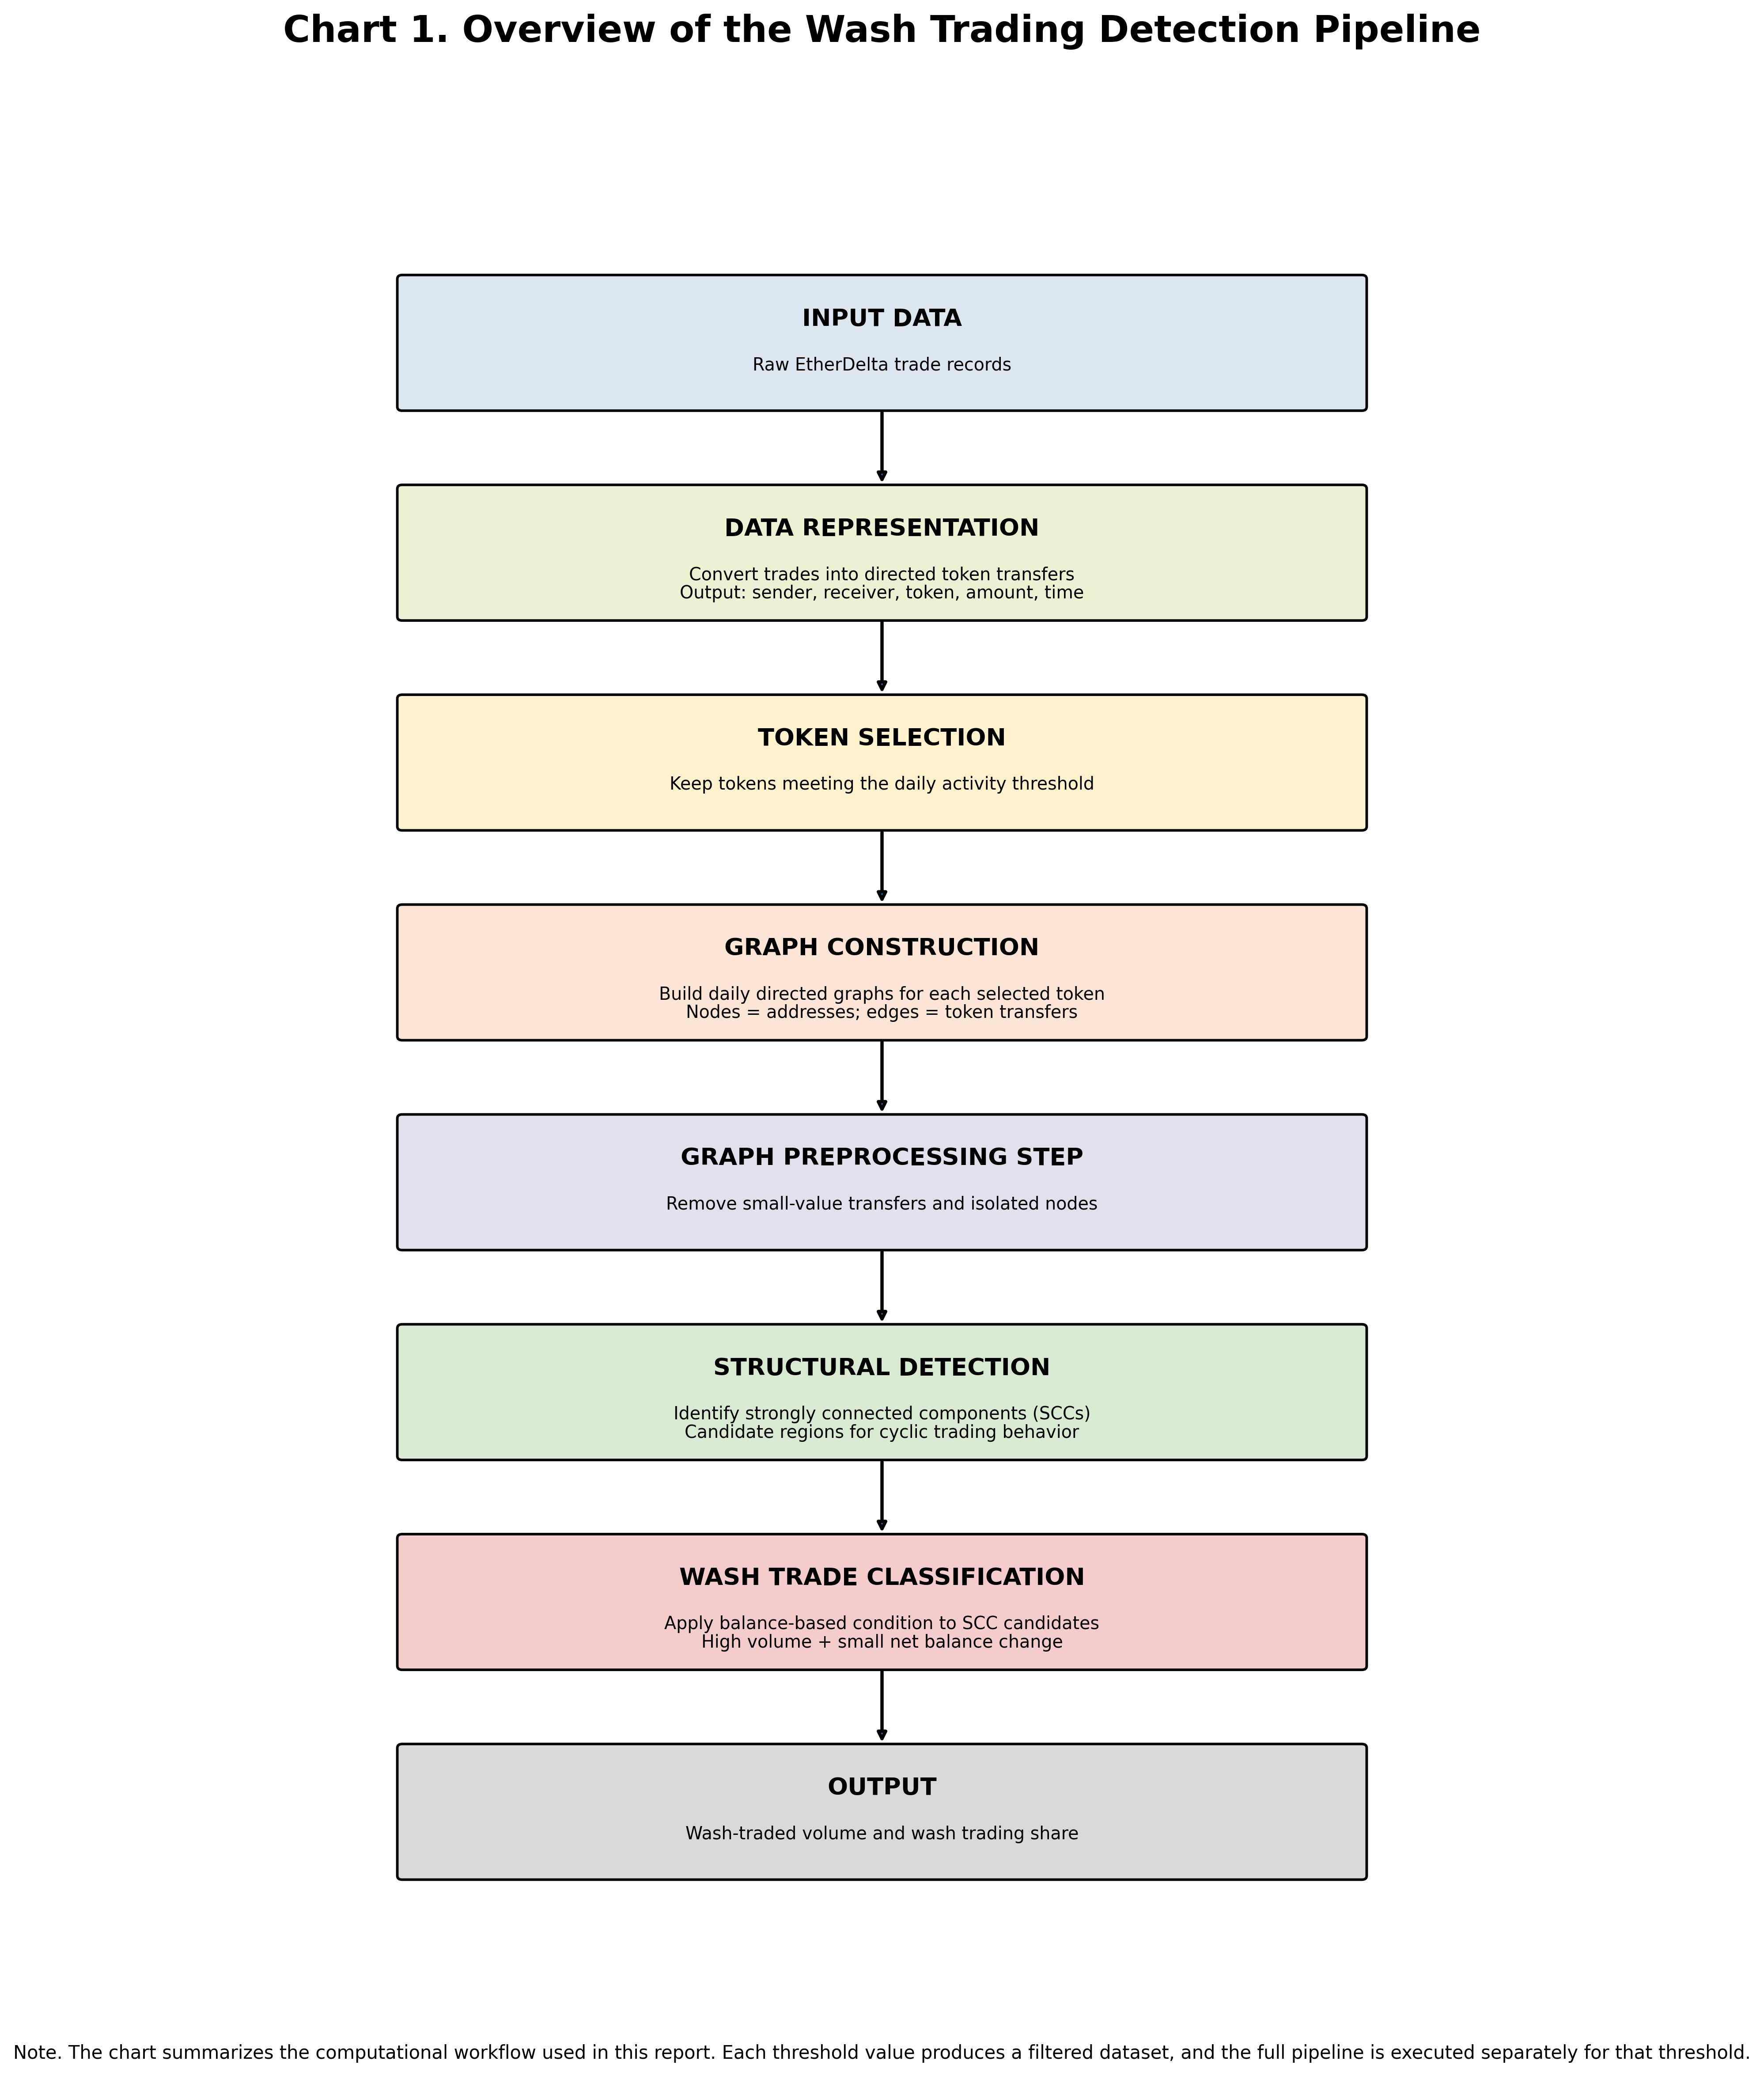
\includegraphics[width=0.8\textwidth, height=18cm]{Chart_1_Overview_of_the_Wash_Trading_Detection_Pipeline}
    \caption{Wash Trading Detection Pipeline}
    \label{fig:my_image}
\end{figure}

\clearpage % Pushes the image out and forces a page break

		\section{Dataset Description}
The analysis uses the EtherDeltaTrades-preprocessed dataset, which contains trade-level records from the EtherDelta decentralized exchange [11]. We selected this dataset because it enables a direct comparison between the methodology of Victor and Weintraud (2021) and the WTEYE framework while controlling for differences in the underlying trading data. Each record includes transaction timestamps, maker and taker addresses, traded token contract addresses, and transaction volumes.\\
EtherDelta operates as an order-book-based decentralized exchange. In this structure, the maker address corresponds to the participant who creates a trading order, while the taker address corresponds to the participant who accepts and executes an existing order. These addresses represent the interacting parties involved in each trade.\\
All blockchain addresses are converted to lowercase to ensure consistency during graph construction and address matching.
The analysis focuses exclusively on ERC20 token transactions [8], [12]. Trades involving Ether (ETH) are excluded because ETH does not follow the ERC20 token transfer standard used by the WTEYE framework [2], [12]. As a result, transactions involving Token–ETH trading pairs are not included in the analysis. Restricting the dataset to ERC20 token transfers ensures that all transactions can be represented consistently as directed token-transfer relationships within the graph structure.\\


	\section{Trade-to-Transfer Conversion}
The original EtherDelta dataset records trading activity as exchange transactions between market participants. However, the WTEYE framework operates on token transfer relationships rather than raw trade records. Therefore, the dataset is transformed into a transfer-based representation suitable for graph analysis.\\
For each transaction, token movements are represented as directed transfers between participating addresses. Each transfer record contains:\\
\\
• a sender address,\\
• a receiver address,\\
• a token identifier,\\
• a transfer amount,\\
• and a timestamp.\\
\\
Conceptually, each row in the transformed dataset represents a single token movement between two addresses. This structure allows token flows to be represented as directed edges within a transaction graph.\\
For a given token, the direction of transfer depends on whether the token is bought or sold in the original trade record. If a participant buys a token, the transfer is represented from the seller address to the buyer address using the traded amount. Similarly, if a token is sold, the transfer direction reflects the movement of that token between participating addresses.\\
This transformation converts exchange-level trading records into a standardized token-transfer format used by the WTEYE framework for graph construction, cycle detection, and balance-based wash trading analysis [12].\\

\begin{table}[h!]
\centering
\begin{tabular}{ccccc}
	\hline
	\textbf{timestamp} & \textbf{sender} & \textbf{receiver} & \textbf{token} & \textbf{amount} \\ \hline
	$t_1$ & Address A & Address B & Token X & 100 \\ 
	$t_2$ & Address B & Address C & Token X & 50  \\ 
	$t_3$ & Address C & Address A & Token X & 100 \\ \hline
\end{tabular}
\caption{Example of transformed transfer-based dataset}
\label{table:transformed_dataset}
\end{table}
\textit{Note.}Each row represents a directed token transfer derived from an exchange trade. The transformed dataset provides the standardized input used for graph construction, where addresses become nodes and token transfers become directed edges. 

	\section{Graph Construction}
For each token, transfers are grouped within fixed time windows. In this study, daily windows are used. Within each window, a directed graph is constructed. \\
In this graph, nodes represent addresses and edges represent token transfers. Each edge corresponds to a transfer from one address to another. This representation allows trading activity to be analyzed as a network.
The use of fixed time windows serves both computational and analytical purposes in large transaction-network analysis [8], [13]. Constructing a single graph over the entire dataset would produce very large and densely connected structures, increasing computational complexity during graph analysis and SCC detection. Dividing transactions into daily windows reduces graph size and improves processing efficiency.\\
Time-windowing also helps capture the short-term nature of wash trading behavior. Coordinated trading activity often occurs within relatively concentrated periods of time, where traders repeatedly exchange assets to inflate apparent market activity. Analyzing transactions within daily intervals therefore helps isolate temporally localized trading patterns.\\
In addition, fixed time windows reduce the formation of artificial graph connections between transactions that occur far apart in time. Without segmentation, addresses involved in unrelated historical trades may become connected within the same graph structure, potentially distorting SCC formation and cycle detection.\\
However, this approach also introduces limitations. Wash trading activity that spans multiple time windows may be separated into different graphs, reducing the visibility of larger coordinated structures. Furthermore, the choice of window size represents a modeling assumption, and different window lengths may produce different graph structures and wash trading estimates.\\

	\section{Graph Preprocessing}
The constructed graphs are simplified before analysis through a preprocessing step. Small-value transfers are removed to reduce noise and improve graph quality [12]. In this study, a transfer is classified as a small-value transfer if its token amount falls below $10^{-6}$ tokens. This threshold corresponds to the parameter used in the implementation to remove extremely small transfers that are unlikely to represent economically meaningful trading activity.\\
Removing very small transfers helps eliminate insignificant or potentially noisy transaction activity, such as dust transfers or automated micro-transactions that may not represent meaningful trading behavior. These transfers can artificially increase graph density by introducing weak or irrelevant connections between addresses.
The removal of small-value transfers also improves computational efficiency by reducing the number of graph edges and simplifying SCC detection. In addition, filtering these transfers helps reduce the formation of spurious cyclic structures that may otherwise affect wash-trading classification.\\
This preprocessing step is particularly important for the balance-based condition used in the WTEYE framework. Extremely small transfers may artificially increase total traded volume while contributing little to actual balance changes. As a result, retaining such transfers could distort the balance ratio used for wash-trade detection and make transaction patterns appear more balanced than they truly are.
The removal of small-value transfers significantly affects graph size and structure. Without filtering, the transaction graph may contain a large number of additional edges created by economically insignificant transfers. These edges increase graph density and may generate weak or artificial connections between addresses. As a result, SCC detection becomes computationally more expensive and potentially more sensitive to noisy transaction activity.\\
After filtering small transfers, the graph becomes sparser and more focused on economically meaningful interactions. This reduction in graph size improves computational efficiency and helps isolate stronger cyclic trading structures. However, aggressive filtering may also remove smaller coordinated trading patterns, potentially excluding some forms of wash trading activity from the analysis.
After filtering small transfers, nodes with no incoming or outgoing edges are iteratively removed. This pruning process ensures that the analysis focuses on connected structures that may represent coordinated trading activity.\\
However, this approach also introduces limitations. If the filtering threshold is set too high, smaller but potentially meaningful trading patterns may be removed from the analysis. Therefore, preprocessing thresholds themselves may influence the final wash trading estimates.\\


	\section{Strongly Connected Components(SCCs) Detection}
After preprocessing, strongly connected components (SCCs) are identified in the transaction graph. An SCC is a group of nodes in which every node can reach every other node through directed transaction paths.\\
In the context of blockchain transactions, nodes represent addresses and edges represent token transfers. An SCC therefore represents a group of addresses connected through repeated chains of transactions. These structures are important because wash trading often involves circular trading activity among coordinated addresses.\\
SCCs are closely related to cycles, but the two concepts are not identical. A cycle represents a single closed transaction loop, whereas an SCC may contain multiple overlapping cycles within a larger connected structure. As a result, SCC detection captures broader patterns of coordinated trading behavior than simple cycle detection alone.\\
For example, a transaction sequence such as: \[ A \rightarrow B \rightarrow C \rightarrow A \] represents a single simple cycle involving exactly one closed loop.\\

\newpage

In contrast, an SCC can be illustrated as a directed subgraph in which all addresses are mutually reachable through directed transaction paths:

\begin{figure}[htbp] % h=here, t=top, b=bottom, p=page
    \centering
    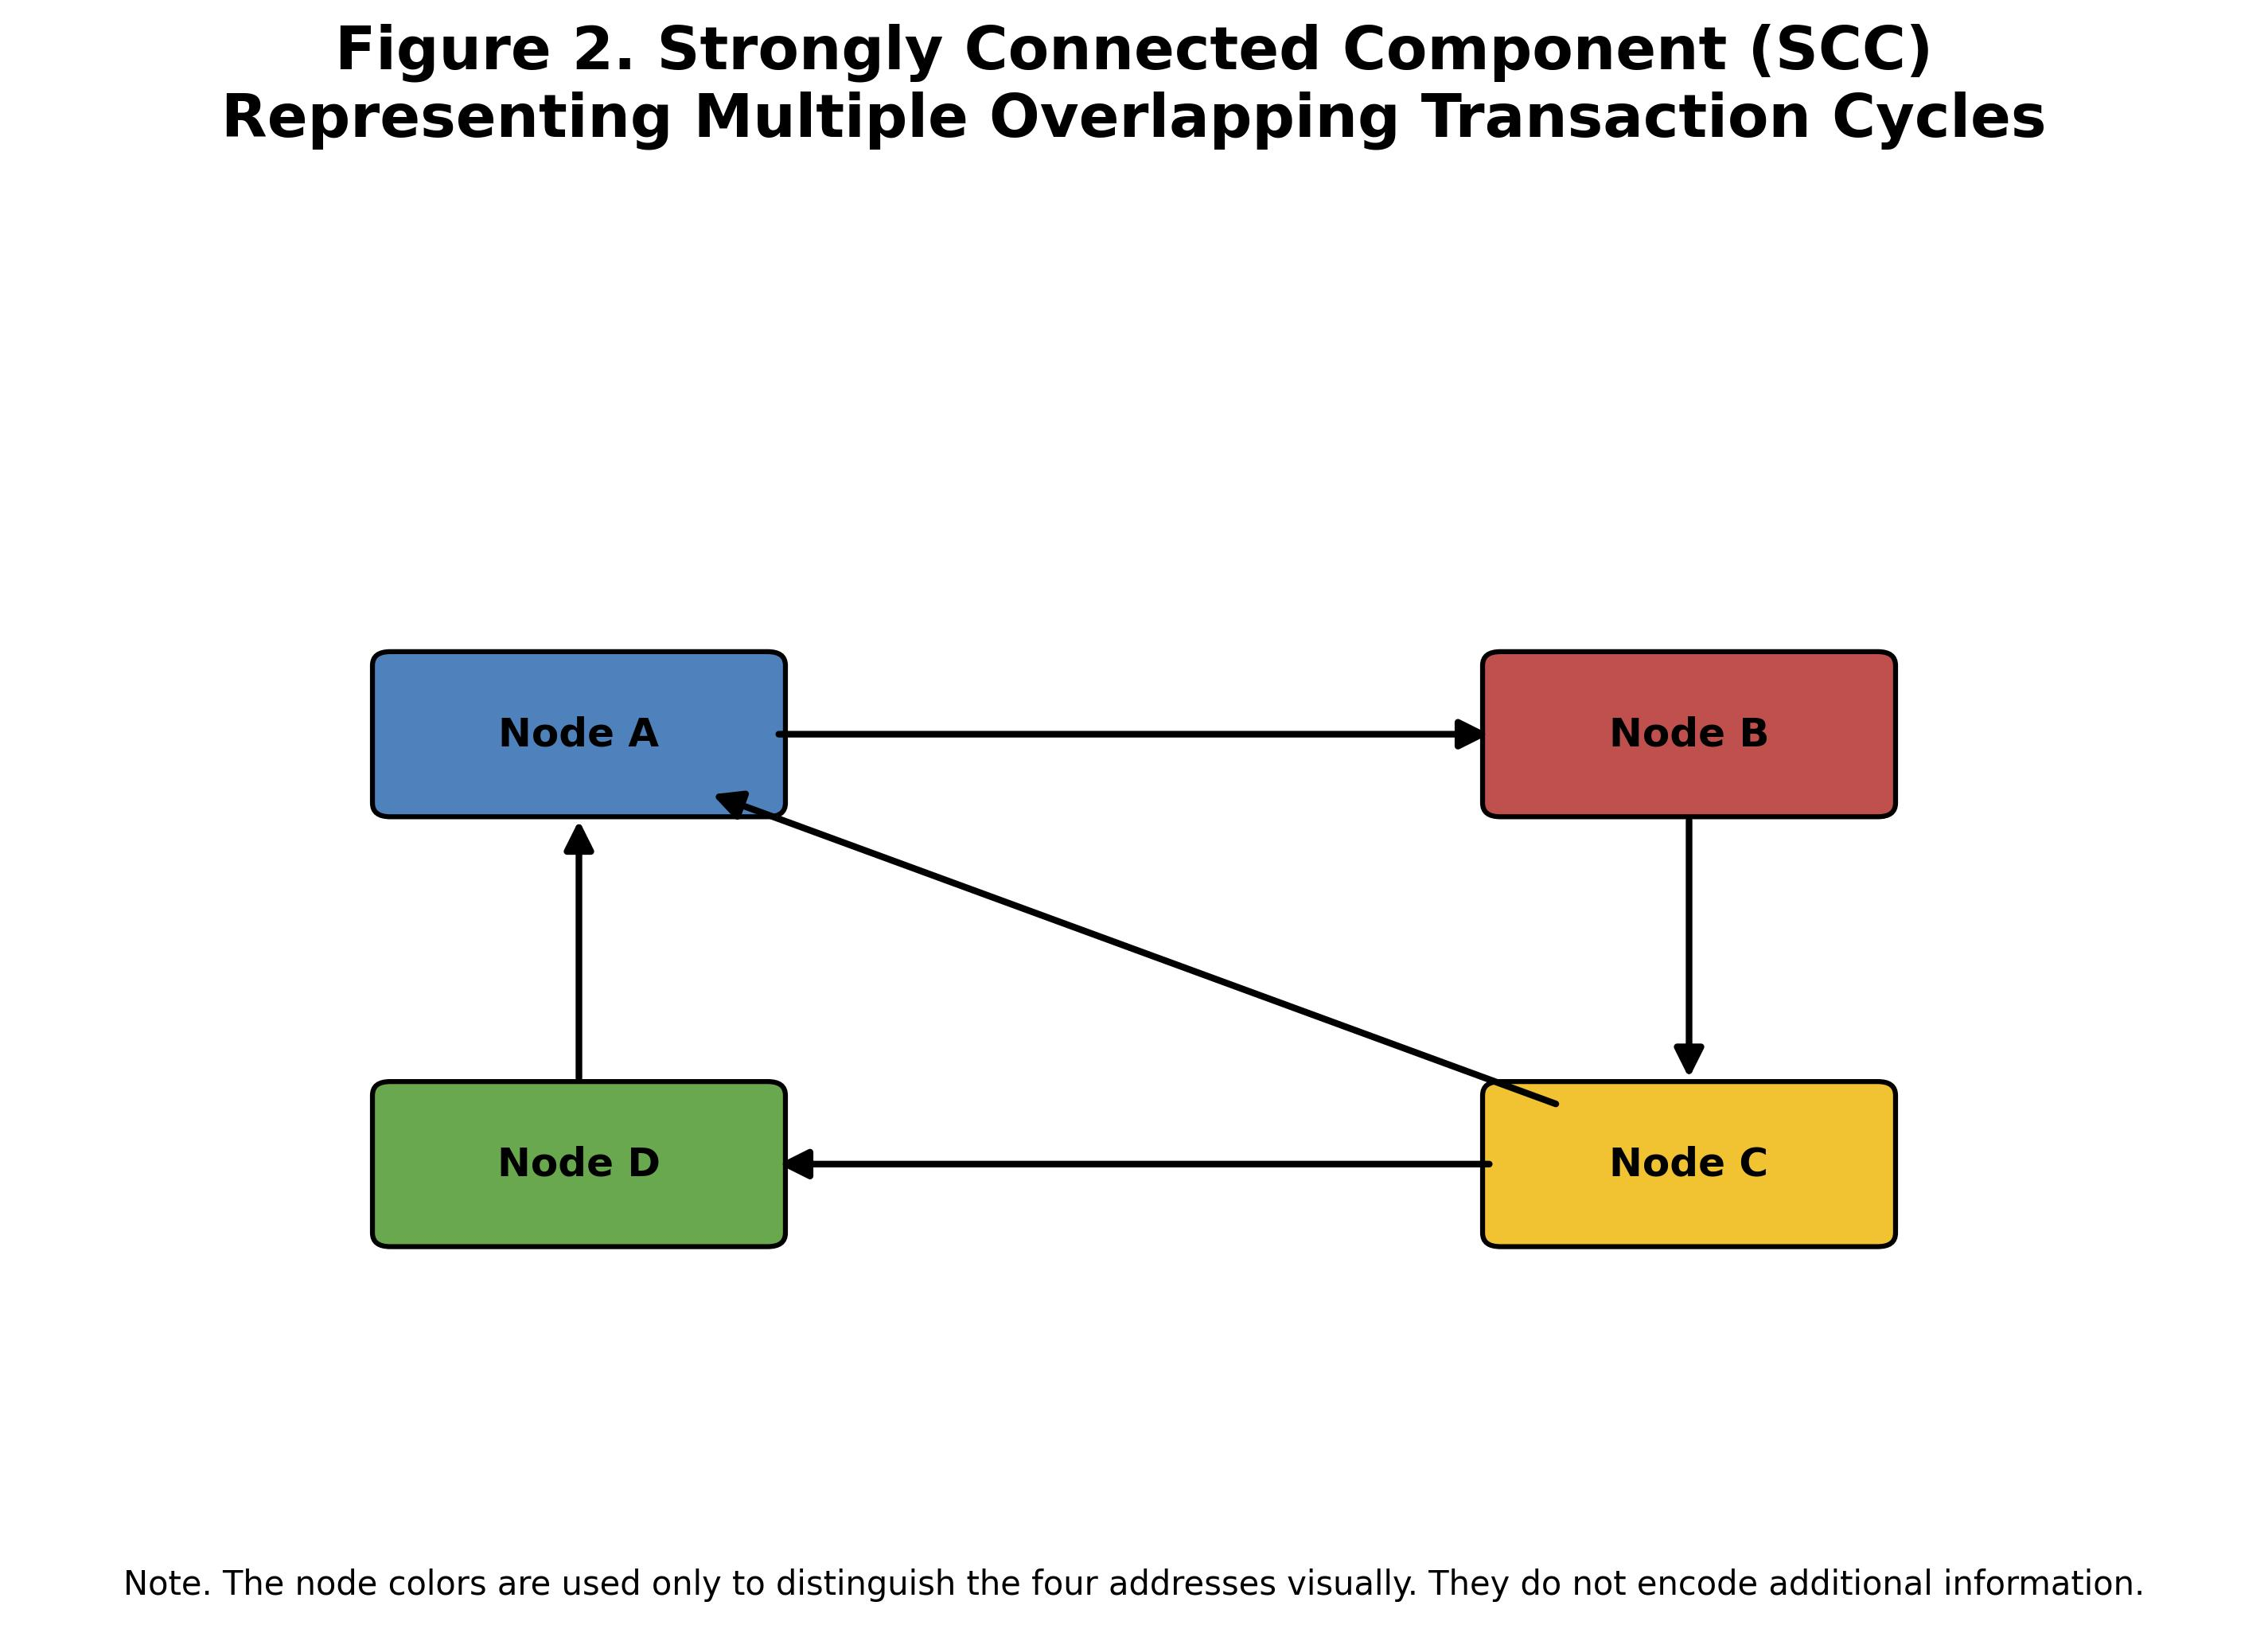
\includegraphics[width=01.0\textwidth]{Figure 2. Strongly Connected Component (SCC) Representing Multiple Overlapping Transaction Cycles}
    \caption{Strongly Connected Components}
    \label{fig:my_image}
\end{figure}


In this example, the arrows represent directed token transfers between addresses. The structure contains multiple closed transaction routes, for example:\\
\\
•	A → B → C → D → A \\
•	A → B → C → A \\
•	C → D → A → B → C \\
\\
Because multiple routes connect the addresses, each address can reach every other address through directed paths. The entire set of addresses therefore forms one strongly connected component.\\
Because wash trading frequently involves repeated exchanges among groups of addresses rather than isolated transaction loops, SCC detection provides a useful method for identifying candidate structures for further wash-trading analysis [5], [11].\\
SCC detection is performed using depth-first-search-based graph traversal algorithms implemented in the igraph library and standard graph decomposition methods [13]. These algorithms identify groups of nodes that are mutually reachable through directed paths.\\
Compared to direct cycle enumeration, SCC decomposition provides a computationally efficient method for identifying coordinated cyclic structures within large transaction graphs. This makes it suitable for analyzing high-volume blockchain transaction networks

	\section{Volume-Based Wash Trade Detection}

For each SCC, the method evaluates whether the observed trading activity satisfies the characteristics of wash trading. The key idea is that wash traders generate trading volume while maintaining a near-neutral position.\\
The balance-based condition evaluates whether trading activity produces substantial changes in token ownership. For each SCC, the method compares the initial and final token balances of all participating addresses.\\
Formally, $S^{(0)}$ and $S^{(m)}$ represent the vectors of token balances before and after the observed transactions within the SCC. The difference between these vectors measures how much token ownership changes during trading activity.\\
The notation $\lVert \cdot \rVert_1$  denotes the $L_1$  norm, which computes the sum of absolute balance differences across all participating addresses. Absolute values are used to prevent gains and losses from canceling each other artificially.\\
The denominator $2V_{\text{total}}$ normalizes the balance deviation relative to the total traded volume. The factor of two appears because each token transfer simultaneously decreases one address balance and increases another. As a result, the total absolute balance movement across all addresses equals twice the transferred volume. The factor of two appears because each token transfer simultaneously decreases one address balance and increases another. As a result, the total absolute balance movement across all addresses equals twice the transferred volume.\\
Wash trading is characterized by large trading volume combined with relatively small net balance changes [12]. Therefore, if the normalized balance deviation remains below the tolerance threshold $\Delta$, the observed trading behavior is classified as potential wash trading.\\
\\
Formally, the condition is defined as:\\
\\
\begin{equation}
    \frac{\lVert S^{(m)} - S^{(0)} \rVert}{2V_{\text{total}}} < \Delta
    \label{eq:volume_bound}
\end{equation}
where:\\
\\
•	$S^{(0)}$ and $S^{(m)}$  represent the initial and final balance vectors,\\
•	$V_{\text{total}}$  denotes total traded volume,\\
•	and $\Delta$ represents the tolerance threshold.\\
\\
Following the WTEYE framework, the tolerance parameter is set to 10\% [12].
	\section{Token-Level Filtering}
This study introduces an additional filtering step before graph construction. Only tokens that appear in at least X transactions within a given day are included in the analysis.\\
The token-level activity threshold is introduced to evaluate whether wash trading estimates are sensitive to token selection criteria. Previous studies detect wash trading using large transaction datasets but do not systematically analyze how filtering tokens by trading activity affects the resulting estimates. By varying the minimum daily token occurrence threshold, this study examines whether wash trading behavior differs across tokens with different activity levels and whether filtering choices significantly influence the measured wash trading share.\\
This parameter controls the level of token activity considered. Low values of X include a large number of tokens, while high values restrict the analysis to highly active tokens. This filtering step is not part of the original WTEYE framework and is introduced specifically to study its effect on wash trading estimates.\\
	\section{Experimental Design}
To evaluate the impact of the filtering parameter, the threshold X is varied from 50 to 200 in increments of 5. For each value of X, the full detection pipeline is executed independently.\\
For each run, the total analyzed token volume and the wash-traded volume are computed. The wash trading share is then calculated as:\\
\begin{equation}
    \text{Wash Trading Share} = \frac{\text{Wash-Traded Volume}}{\text{Total Analyzed Volume}}
    \label{eq:wash_trading_share}
\end{equation}
By comparing results across different threshold values, the analysis evaluates how sensitive wash trading estimates are to token-level filtering choices.

	\chapter{Analysis}
This section presents the empirical analysis of wash trading under varying token-level activity thresholds. The goal is to evaluate how the estimated wash trading share changes as the minimum daily occurrence parameter is varied. The analysis follows the methodology described in Section 3 and applies the WTEYE framework to each filtered dataset [12].\\
The analysis focuses on whether token-level filtering influences the measured wash trading share. By systematically varying the minimum daily token occurrence threshold, the study examines how preprocessing decisions affect the composition of the dataset and the resulting wash trading estimates.
	\section{Experimental Setup}
The analysis varies the minimum daily token occurrence threshold from 50 to 200 in increments of 5. For each value of $X$ , the dataset is filtered to include only tokens that meet the required activity level.\\
The full detection pipeline is then applied to each filtered dataset. This includes:\\
\\
•	trade-to-transfer conversion,\\
•	graph construction,\\
•	graph preprocessing,\\
•	SCC detection,\\
•	and volume-based wash trade classification [12].\\
\\
The detection follows the balance-based condition defined in Section 3.7 [12].\\
For each threshold, two quantities are computed:\\
\\
•	total analysed token volume,\\
•	wash-traded token volume.\\
\\
The wash trading share has already been defined previously in Equation \ref{eq:wash_trading_share}:\\
\begin{equation}
    \text{Wash Trading Share} = \frac{\text{Wash-Traded Volume}}{\text{Total Analyzed Volume}}
    \tag{\ref{eq:wash_trading_share}}
\end{equation}
This metric is consistent with prior work on wash trading quantification [11],[12].
	\section{Results}
The results show that wash trading estimates vary significantly across different threshold values, consistent with prior studies demonstrating heterogeneous wash trading behavior across cryptocurrency markets [11], [12]. The relationship between the threshold and the wash trading share is non-linear and exhibits distinct regions of behavior.\\
For thresholds between 50 and 80, the wash trading share remains close to zero. In contrast, thresholds between approximately 90 and 120 produce substantially higher values, reaching approximately 70\%. For thresholds between 125 and 145, the wash trading share decreases to around 13\%. For thresholds above 150, the values drop below 1\% and stabilize near zero.\\
These results indicate that wash trading is not uniformly distributed across tokens. Instead, the concentration of wash trading appears to vary depending on the level of token activity included in the analysis.
\begin{table}[h!]
\centering
\begin{tabular}{cc}
	\hline
	\textbf{Threshold Range} & \textbf{Approximate Wash Trading Share} \\ \hline
	$50-80$    & $\sim 0.000002\%$ \\ 
	$90-120$   & $\sim 71\%$       \\ 
	$125-145$  & $\sim 13\%$       \\ 
	$150-175$  & $\sim 0.4\%$      \\ 
	$>200$      & $\sim 0.0527\%$   \\ \hline
\end{tabular}
\caption{Wash trading share across token-level activity thresholds}
\label{table:wash_trading_shares}
\end{table}
	\section{Interpretation}
Differences in token activity levels can explain the observed pattern. At low thresholds, the dataset contains many low-activity tokens. These tokens typically have sparse trading activity and limited transaction volume. As a result, they rarely form the cyclic structures required for wash trading detection. Consequently, the detected wash trading volume remains negligible relative to the total volume.
At intermediate thresholds, the dataset includes tokens with moderate activity levels. These tokens have sufficient transaction volume to form cycles but remain small enough to be influenced by a limited number of participants. This creates favorable conditions for coordinated trading behavior. As a result, wash trading becomes concentrated in this range, leading to a sharp increase in the measured wash trading share.\\
At higher thresholds, the dataset is restricted to highly active tokens. These tokens typically involve a larger number of independent participants and more diverse trading patterns. As a result, the relative impact of coordinated wash trading decreases, and the measured share declines.\\
This interpretation is consistent with the assumption that wash trading involves cyclic trading patterns combined with balance-neutral behavior [12].\\

\begin{figure}[htbp] % h=here, t=top, b=bottom, p=page
    \centering
    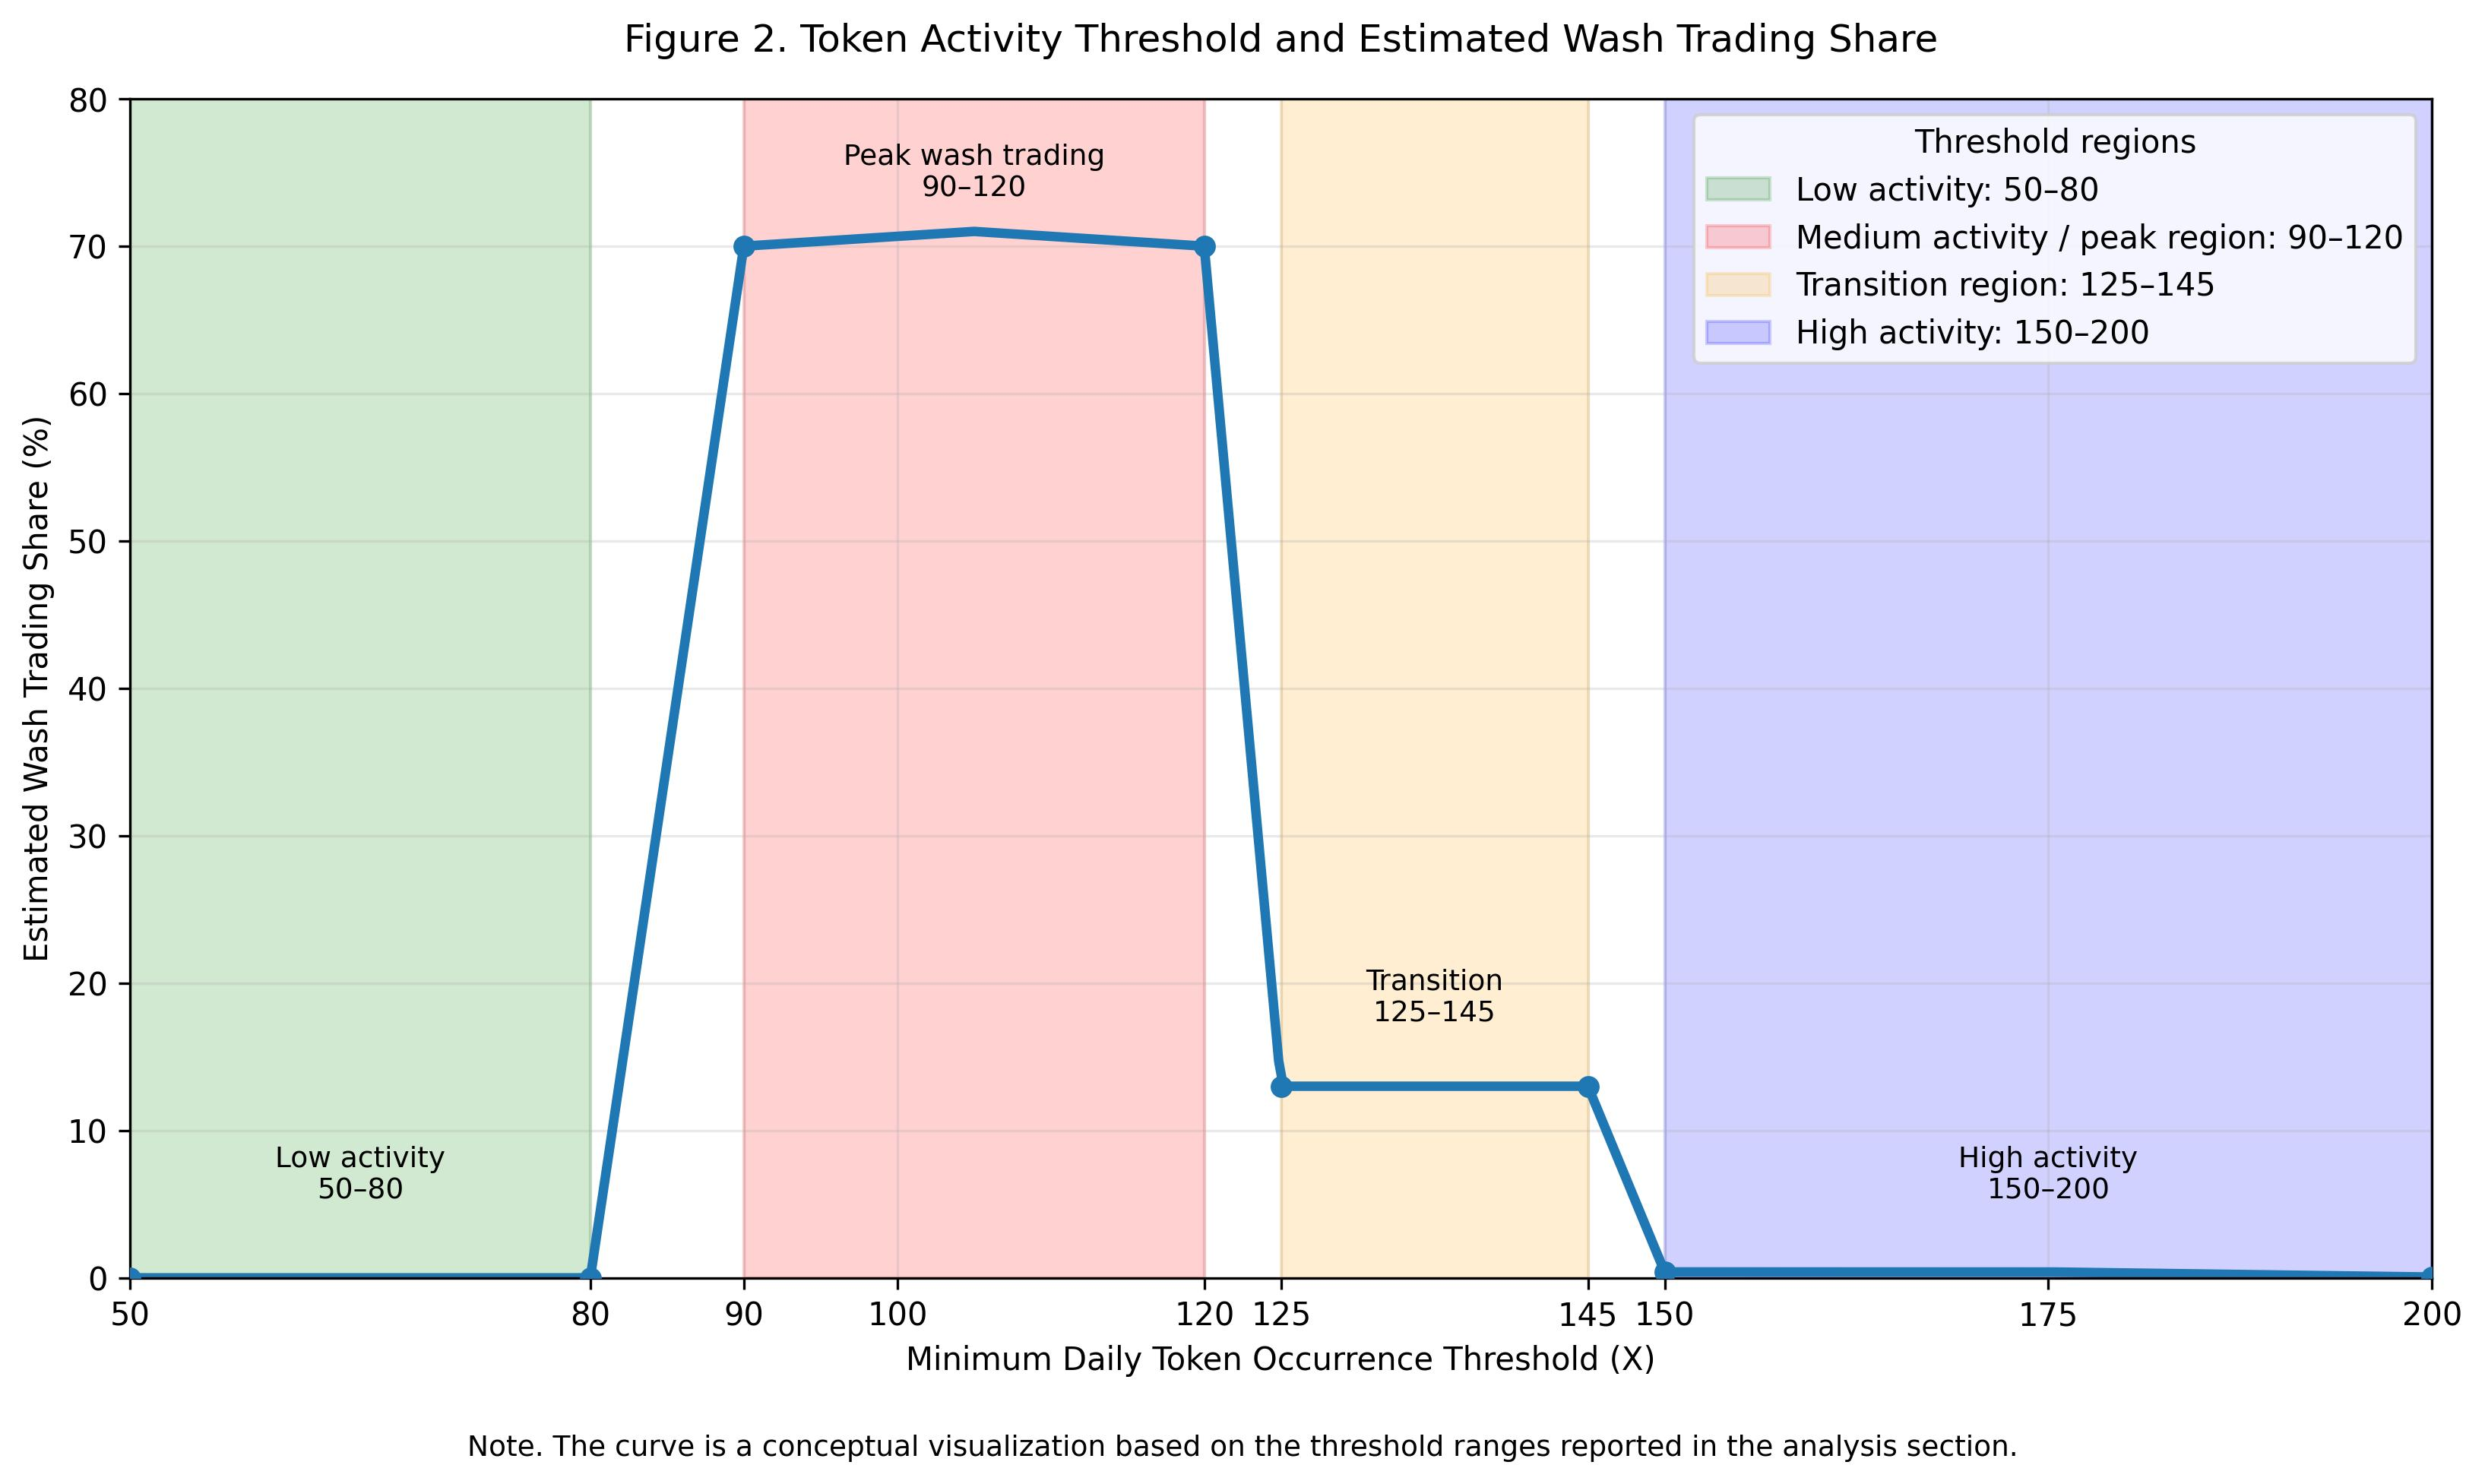
\includegraphics[width=0.8\textwidth]{Figure_3_Token_Activity_Thresholds_Numbered}
    \caption{Threshold Range Vs Wash Share Activity}
    \label{fig:my_image}
\end{figure}
\textit{Note.} The colored zones are illustrative and are intended to distinguish the three behavioural regimes identified in the empirical analysis.
	\section{Sensitivity Analysis}
The results demonstrate that wash trading estimates are highly sensitive to the choice of token-level filtering parameter. Changing the threshold significantly alters both the composition of the dataset and the resulting wash trading share.\\
This finding highlights that wash trading measurements are not solely determined by the detection algorithm. Instead, they also depend on the selection of data included in the analysis. Similar dependencies are implicitly present in prior work, where filtering steps are applied either explicitly or implicitly [11], [12].\\
The analysis therefore suggests that preprocessing choices represent an important methodological factor in graph-based wash trading detection [11], [12]. Different filtering decisions may produce substantially different estimates, even when the same detection framework is applied [11], [12].
	\section{Implications}
The sensitivity of the results has important implications for interpreting wash trading estimates. Reported values may vary depending on how tokens or transactions are selected prior to analysis.\\
In particular, methods that rely on fixed thresholds or implicit filtering decisions may produce results that are not directly comparable. This suggests that wash trading estimates should be interpreted in the context of the underlying data selection process.\\
The findings also indicate that token activity level is an important factor in determining susceptibility to wash trading. Tokens with moderate activity appear to be more vulnerable to manipulation than both low-activity and highly active tokens.\\
More broadly, the results demonstrate that graph-based wash trading analysis is influenced not only by detection algorithms but also by preprocessing design choices. Future studies may therefore benefit from reporting filtering parameters more explicitly and evaluating their influence systematically [11], [12].
	\section{Limitations}
This analysis has several limitations. First, it is based on a single dataset derived from EtherDelta. The observed patterns may not generalize to other exchanges or market structures.\\
Second, the analysis relies on the WTEYE detection framework, which assumes that wash trading is characterized by cyclic structures and balance-neutral behavior [12]. While this assumption captures many cases, it may not detect all forms of manipulation.\\
Third, the results depend on the chosen threshold range. Different parameter ranges may produce different patterns. As a result, the conclusions should be interpreted as indicative rather than definitive.\\
In addition, the use of daily time windows and graph preprocessing introduces further modeling assumptions. Different window sizes, filtering thresholds, or preprocessing strategies may alter graph structure and influence SCC detection results.
	\subsection{Computational and Data Challenges}
During the analysis, several computational and data-related challenges were encountered. One major issue involved incomplete or inconsistent token decimal information for certain ERC20 tokens. Because token transfer values depend on token-specific decimal scaling, missing or incorrect decimal mappings occasionally produced unrealistic transaction volumes and distorted wash trading estimates. This issue was addressed by extending and correcting the token-decimal mapping used during preprocessing.\\
The analysis also revealed strong sensitivity to preprocessing and filtering choices. Certain threshold values produced sparse transaction graphs or near-empty datasets, occasionally resulting in unstable outputs or negligible wash trading estimates. These observations reinforced the importance of systematically evaluating token-level filtering effects.\\
In addition, graph-based blockchain analysis introduced computational challenges due to the large size of transaction networks. SCC detection and graph traversal became increasingly expensive as graph density increased. To improve computational efficiency, the analysis used daily time-window segmentation, graph pruning, and small-value transfer filtering to reduce graph complexity [8], [13].\\
The full analysis required repeated execution of the wash trading detection pipeline across multiple threshold values. As a result, computational cost increased substantially with graph size and transaction density. These challenges highlight the practical importance of preprocessing and graph simplification in large-scale blockchain transaction analysis [8], [12], [13].

	\chapter{Conclusion}
This study examined wash trading in decentralized cryptocurrency markets using the WTEYE framework [12]. The analysis applied this method to a preprocessed EtherDelta dataset and introduced a token-level activity threshold to evaluate how data filtering influences wash trading estimates.\\
The results show that wash trading is not uniformly distributed across tokens. Instead, wash trading activity appears to concentrate within a specific range of token activity levels. Tokens with moderate activity exhibited substantially higher wash trading shares than both low-activity and highly active tokens.\\
More importantly, the analysis demonstrates that wash trading estimates are highly sensitive to preprocessing and filtering choices. Varying the minimum daily token occurrence threshold significantly changed both the composition of the analyzed dataset and the resulting wash trading measurements. These findings indicate that empirical estimates of wash trading are influenced not only by the detection framework itself but also by methodological decisions regarding data selection and preprocessing.\\
The main contribution of this report is therefore to show that token-level activity filtering can substantially affect graph-based wash trading estimates in decentralized exchange data. By systematically varying the filtering threshold, this study provides additional insight into how preprocessing assumptions influence the interpretation of empirical blockchain analyses.\\
These findings highlight the importance of methodological transparency in cryptocurrency market analysis [11], [12]. Studies that apply different filtering strategies or preprocessing assumptions may produce results that are not directly comparable, even when similar detection methods are used.\\
Future research could extend this analysis to additional decentralized exchanges, alternative graph-based detection frameworks, and different blockchain ecosystems [6], [11]. Further work could also examine how other preprocessing choices, such as time-window selection, graph pruning strategies, or transaction-value thresholds, influence wash trading detection outcomes. Such extensions may contribute to a more reproducible and methodologically robust understanding of manipulation in decentralized financial markets [6], [11], [12].
\clearpage
\printbibliography[heading=bibintoc] % Renders bibliography and appends to Table of Contents

% =========================================================
% APPENDIX SECTION
% =========================================================
\clearpage

\appendix % Toggles the document numbering engine to Appendix mode (A, B, C...)

\addchap{Appendix} % Creates an unnumbered Appendix heading that links to the TOC
\thispagestyle{plain}

The auxiliary resources, underlying datasets, and implementation source code for this investigation are publicly accessible via the following repositories:

\begin{itemize}
    \item \textbf{Dataset:} The preprocessed and transformed trading data is hosted on  \href{https://zenodo.org/records/4540223}{Zenodo}
    \item \textbf{Source Code:} The complete graph analysis implementation script repository is hosted on the \href{https://git.hs-mittweida.de/frafique/preliminary-investigation-of-wash-trading-detection-on-etherdelta-using-graph-based-methods.git}{HSMW GitLab}  and  \href{https://git.hs-mittweida.de/frafique/preliminary-investigation-of-wash-trading-detection-on-etherdelta-using-graph-based-methods.git}{here}
\end{itemize}

\end{document}